% File: solutions/ex4.tex

\begin{soluzione}{4}
    Il processo di campionamento di un segnale nel tempo causa una \textbf{periodicizzazione} del suo spettro nel dominio della frequenza. Lo spettro del segnale campionato, $\tilde{X}(f)$, è una somma infinita di repliche dello spettro originale, $X(f)$, scalate in ampiezza e centrate a multipli interi della frequenza di campionamento $f_s$.

    \subsubsection*{1. Analisi dei Parametri e Condizione di Aliasing}
    I dati del problema sono:
    \begin{itemize}
        \item Massima frequenza del segnale: $B = 100$ Hz.
        \item Frequenza di campionamento: $f_s = 300$ Hz.
    \end{itemize}
    Verifichiamo la condizione di Nyquist per assenza di aliasing:
    \[
        f_s \ge 2B \implies 300 \text{ Hz} \ge 2 \cdot 100 \text{ Hz} \implies 300 \text{ Hz} \ge 200 \text{ Hz}
    \]
    La condizione è soddisfatta. Ciò significa che le repliche spettrali non si sovrapporranno e il segnale potrà essere ricostruito perfettamente.

    \subsubsection*{2. Struttura dello Spettro Campionato}
    La formula generale per lo spettro campionato è:
    \[
        \tilde{X}(f) = \frac{1}{T} \sum_{k=-\infty}^{\infty} X(f - k f_s)
    \]
    Dove $T = 1/f_s = 1/300$ s.
    
    Il fattore di scala per l'ampiezza è quindi $1/T = f_s = 300$. Poiché il picco dello spettro originale $X(f)$ è 1 (a $f=0$), il picco di ogni replica in $\tilde{X}(f)$ sarà $1 \cdot 300 = 300$.
    
    Le repliche saranno centrate a $f = k \cdot f_s = k \cdot 300$ Hz. Per l'intervallo richiesto (da -500 a 500 Hz), vedremo tre repliche:
    \begin{itemize}
        \item \textbf{Per k=0:} Una replica di $X(f)$ centrata a $0$ Hz, che si estende da $-100$ a $100$ Hz.
        \item \textbf{Per k=1:} Una replica di $X(f)$ centrata a $300$ Hz, che si estende da $200$ a $400$ Hz.
        \item \textbf{Per k=-1:} Una replica di $X(f)$ centrata a $-300$ Hz, che si estende da $-400$ a $-200$ Hz.
    \end{itemize}

    \subsubsection*{3. Grafico dello Spettro}
    Di seguito è riportato il grafico qualitativo di $\tilde{X}(f)$.

    \begin{center}
    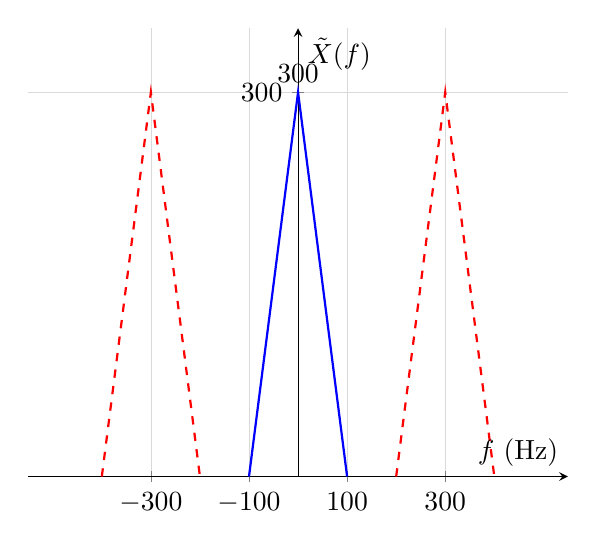
\begin{tikzpicture}
        \begin{axis}[
            axis lines=middle,
            xlabel=$f$ (Hz),
            ylabel=$\tilde{X}(f)$,
            xmin=-550, xmax=550,
            ymin=0, ymax=350,
            xtick={-300, -100, 0, 100, 300},
            ytick={300},
            grid=both,
            grid style={line width=.1pt, draw=gray!30},
            legend pos=outer north east
        ]
        
        % Replica centrale (k=0)
        \addplot[blue, thick] coordinates { (-100, 0) (0, 300) (100, 0) };
        
        % Replica a destra (k=1)
        \addplot[red, thick, dashed] coordinates { (200, 0) (300, 300) (400, 0) };

        % Replica a sinistra (k=-1)
        \addplot[red, thick, dashed] coordinates { (-400, 0) (-300, 300) (-200, 0) };
        
        % Annotazioni
        \node[above] at (axis cs:0, 300) {300};
        \node[below] at (axis cs:0, -10) {$0$};
        \node[below] at (axis cs:300, -10) {$f_s$};
        \node[below] at (axis cs:-300, -10) {$-f_s$};
        
        \end{axis}
    \end{tikzpicture}
    \end{center}
    Il grafico mostra chiaramente la replica centrale (blu) e le due repliche adiacenti (rosse tratteggiate), tutte con ampiezza di picco 300 e separate da uno spazio vuoto, confermando l'assenza di aliasing.
    
\end{soluzione}